\section{Interpolation-Based Compression: FDWZ}\label{sec:SZ3-HOHS}

FDWZ follows the SZ compression framework. Section~\ref{sec:SZ3-HOHS:sz3 interpolation} briefly reviews this framework. Sections~\ref{sec:FDWZ:distance-weighted} and~\ref{sec:FDWZ:multi-tree} describe how FDWZ differs from it, as summarized in Figure~\ref{fig:fdwz-workflow}. Finally, Section~\ref{sec:FDWZ:prediction-locality} compares predictability within an element, along the stored element-index dimension, and across adjacent element boundaries.

\begin{figure}[htb]
    \centering
    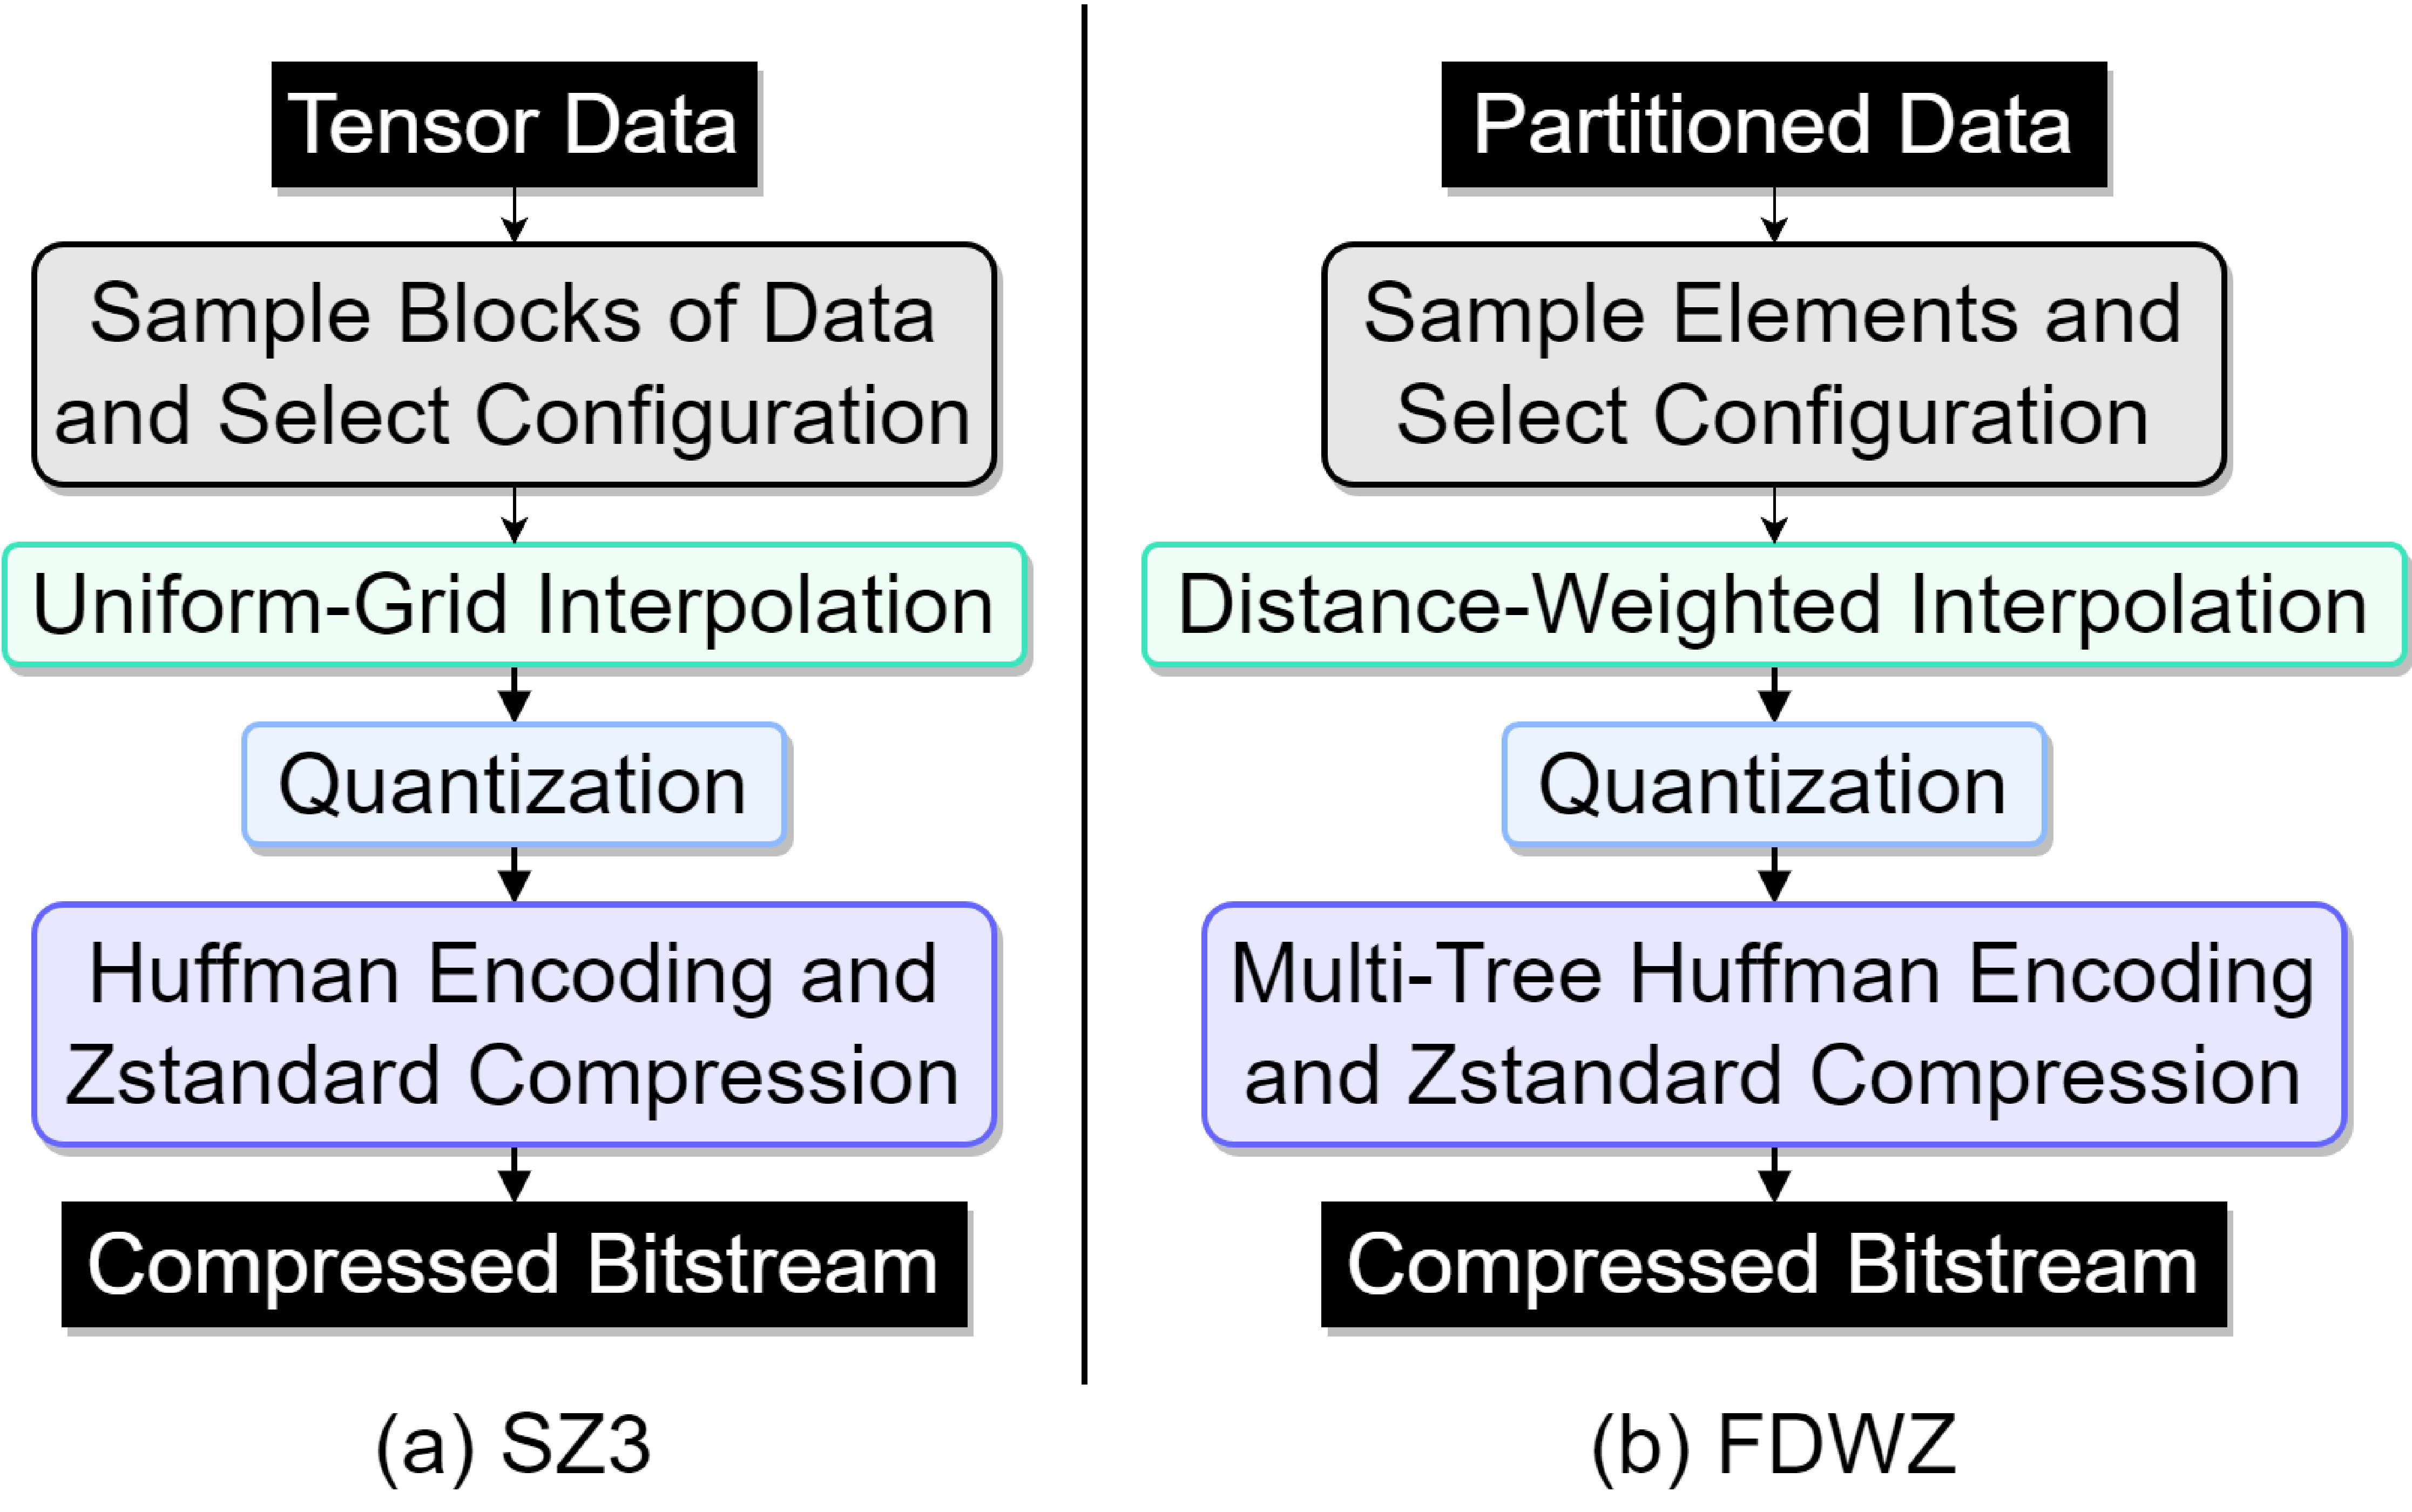
\includegraphics[width=\linewidth]{figs/5/fdwz diagram.pdf}
    \caption{Comparison of standard SZ3 compression on tensor data (left) and FDWZ compression on a high-order element partition (right). FDWZ replaces uniform-grid interpolation with distance-weighted interpolation and single-tree Huffman encoding with multi-tree encoding.}
    \label{fig:fdwz-workflow}
\end{figure}

\subsection{SZ Compression Framework}\label{sec:SZ3-HOHS:sz3 interpolation}

The SZ framework follows a prediction--quantization--encoding pipeline~\cite{tao2017significantly,liang2022sz3}. For each target value, it predicts from previously reconstructed values and quantizes the prediction error under a user-specified error bound. Using reconstructed references keeps the compressor and decompressor synchronized while preserving the pointwise error guarantee. The resulting quantization symbols are encoded using a single Huffman tree followed by Zstandard~\cite{zstd}. Within this pipeline, SZ3 applies multilevel interpolation to a multidimensional array, predicting points level by level and using each reconstructed level as a reference for later levels.

A representative predictor in SZ3 uses cubic interpolation on a uniform array grid. As illustrated in Figure~\ref{fig:cubic-interpolation}(a), it predicts a target by evaluating the cubic polynomial fitted through four reconstructed reference values. On a uniform grid, this yields the fixed Lagrange interpolation weights listed in Table~\ref{tab:cubic-interpolation}.

\subsection{Distance-Weighted Multilevel Interpolation}\label{sec:FDWZ:distance-weighted}

FDWZ adapts this cubic interpolation to the nonuniform spacing of GLL points within each high-order element. This adaptation involves two changes: distance-weighted interpolation and a modified prediction order.

\begin{enumerate}
\item \textit{Distance-Weighted Interpolation}: Because GLL points are nonuniformly spaced, the fixed coefficients used by SZ3 no longer represent the cubic interpolant at the target position. In principle, FDWZ could compute interpolation weights from the physical coordinates of each element. However, repeating this calculation for every target in every element would be expensive. FDWZ therefore computes cubic Lagrange weights from the reference-space coordinates of the target and reference points. Figure~\ref{fig:cubic-interpolation}(b) illustrates such a stencil, and Table~\ref{tab:cubic-interpolation} lists its coordinates and weights. Because all elements with the same polynomial order share these coordinates~\cite{Isoparametric-Mapping}, the resulting weights can be reused across them.
\item \textit{Modified Prediction Order}: SZ3 constructs its multilevel hierarchy by repeatedly selecting the array-index midpoint between two reconstructed endpoints. On a uniform grid, this point is also their geometric midpoint. FDWZ instead selects the unpredicted GLL point closest to the midpoint of the two endpoints in reference space. This choice helps limit the propagation of compression errors to later prediction levels. This order is also computed once per polynomial order and reused across elements.
\end{enumerate}

\begin{figure}[htb]
    \centering
    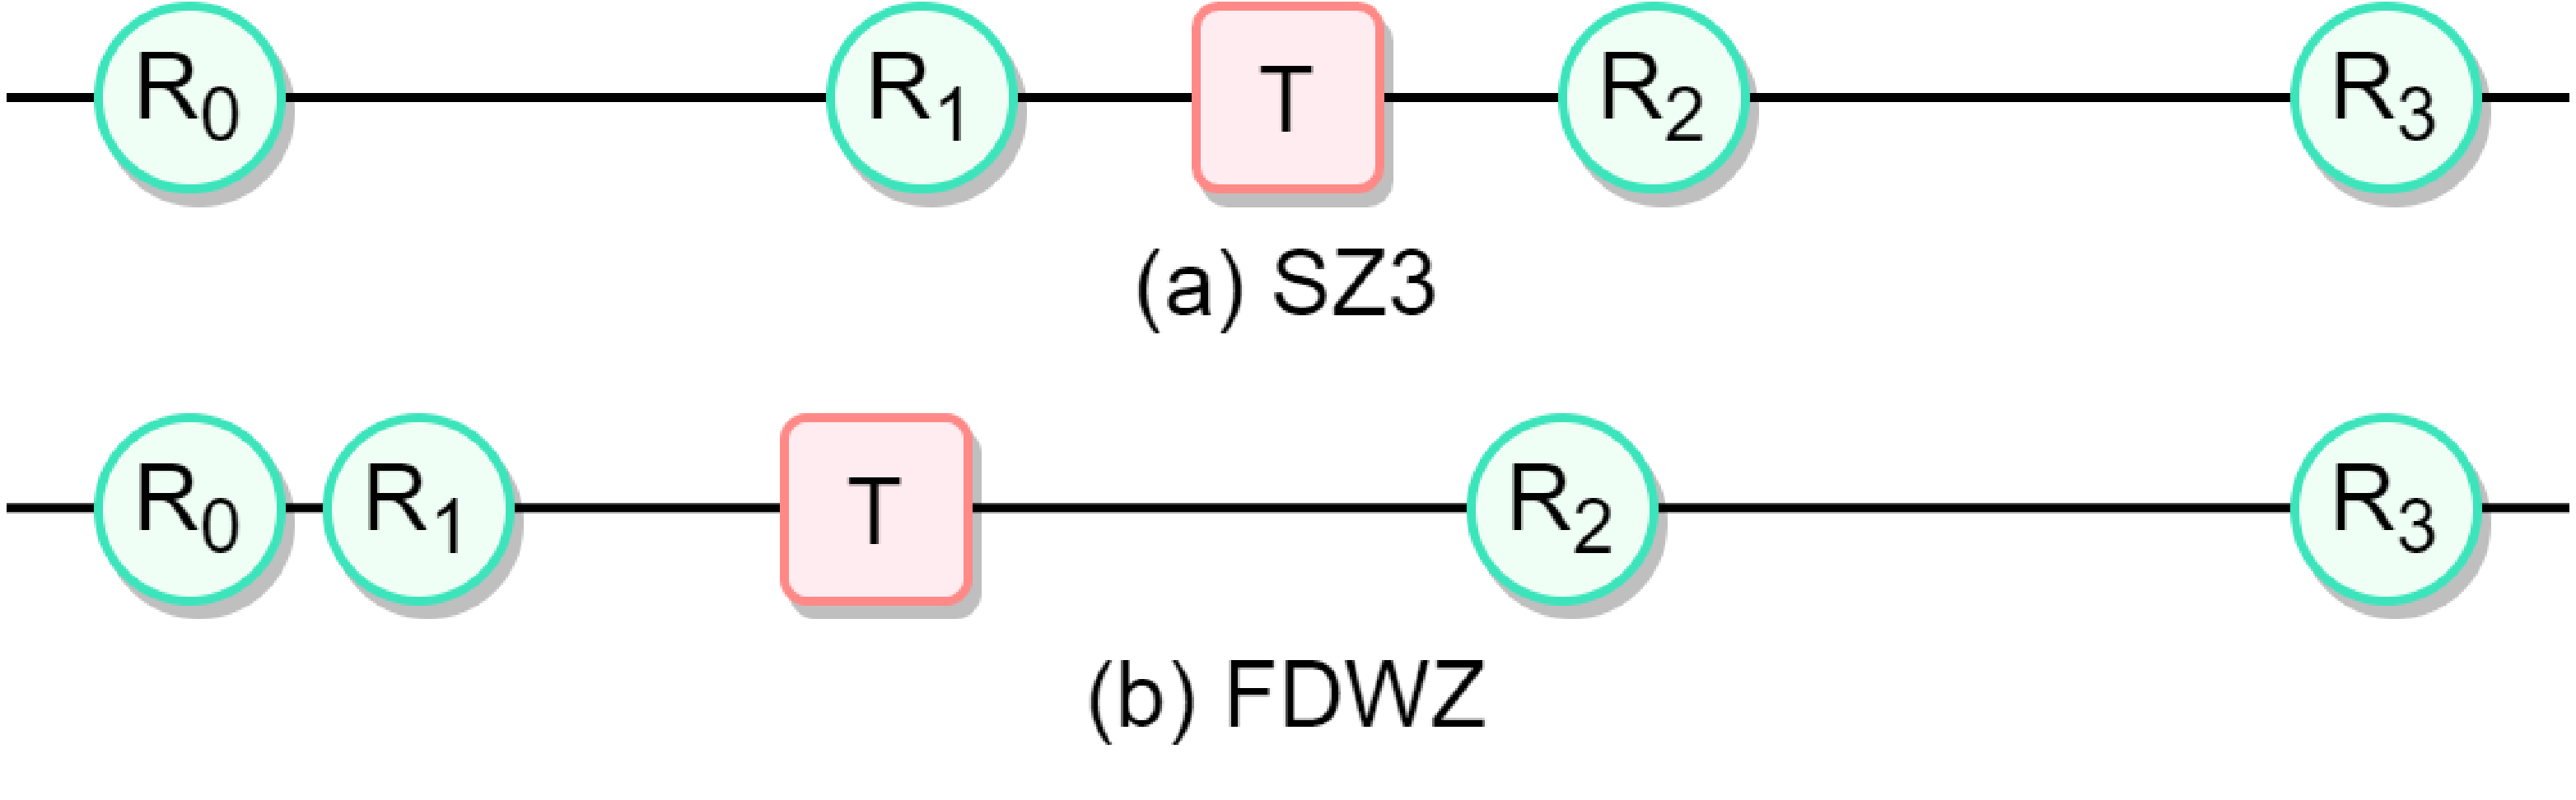
\includegraphics[width=\linewidth]{figs/5/cubic interpolation.pdf}
    \caption{Comparison of cubic interpolation stencils in SZ3 and FDWZ. The target $T$ is predicted from reference points $R_0$--$R_3$.}
    \label{fig:cubic-interpolation}
\end{figure}

\begin{table}[htb]
    \centering
    {\footnotesize
    \setlength{\tabcolsep}{4pt}
    \renewcommand{\arraystretch}{1.05}
    \begin{tabular*}{\columnwidth}{@{\extracolsep{\fill}}lccccc@{}}
        \toprule
        & $R_0$ & $R_1$ & $T$ & $R_2$ & $R_3$ \\
        \midrule
        SZ3: $x/d$ & \textminus3 & \textminus1 & 0 & 1 & 3 \\
        SZ3: $w$ & \textminus0.0625 & 0.5625 & --- & 0.5625 & \textminus0.0625 \\
        FDWZ: $x/a$ & 0 & 0.040 & 0.131 & 0.261 & 0.417 \\
        FDWZ: $w$ & \textminus0.771 & 1.458 & --- & 0.376 & \textminus0.063 \\
        \bottomrule
    \end{tabular*}}
    \caption{Coordinates and cubic interpolation weights in Figure~\ref{fig:cubic-interpolation}. FDWZ coordinates are normalized by the reference-element length $a$; FDWZ values are rounded to three decimal places.}
    \label{tab:cubic-interpolation}
\end{table}

Element-local prediction also provides favorable memory locality. On large regular tensor datasets, SZ3 may perform long-range accesses during multilevel prediction. High-order elements, in contrast, are typically small, often no larger than $10 \times 10 \times 10$, allowing FDWZ to operate primarily on cache-resident data.

\subsection{Multi-tree Huffman Encoding}\label{sec:FDWZ:multi-tree}

Quantization-symbol distributions differ across FDWZ prediction levels. Earlier levels generally use reference points farther from their targets, producing larger prediction errors and a wider distribution of quantization symbols. Later levels use closer reference points and therefore tend to produce smaller errors and symbols that are more concentrated near zero.

Encoding symbols from all levels with one Huffman tree mixes these distributions and yields code lengths that are poorly matched to individual groups. FDWZ therefore aggregates corresponding symbols across elements and encodes them using at most five Huffman trees: one for corner symbols, separate trees for the earliest prediction levels, and one for any remaining levels. This cap retains most of the benefit of distribution-specific coding without excessive codebook overhead. The encoded streams are finally compressed together using Zstandard.

\begin{figure}[htb]
    \centering
    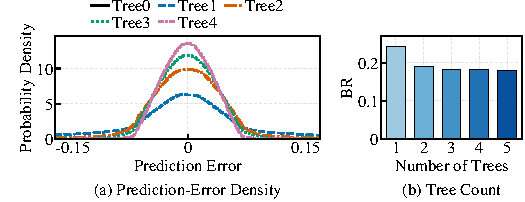
\includegraphics[width=\linewidth]{figs/5/fdwz-tree-ablation.pdf}
    \caption{Impact of multi-tree Huffman encoding on the $P$ field of pb0. (b) Rate--distortion performance using a single Huffman tree and up to five Huffman trees. Across the five error bounds, multi-tree encoding improves the compression ratio by 26.5\% on average.}
    \label{fig:fdwz-tree-ablation}
\end{figure}

\subsection{Comparison of Prediction Locality}\label{sec:FDWZ:prediction-locality}\label{sec:SZ3-HOHS:element_dimension}\label{sec:SZ3-HOHS:cross_element}

\begin{figure}[htb]
    \centering
    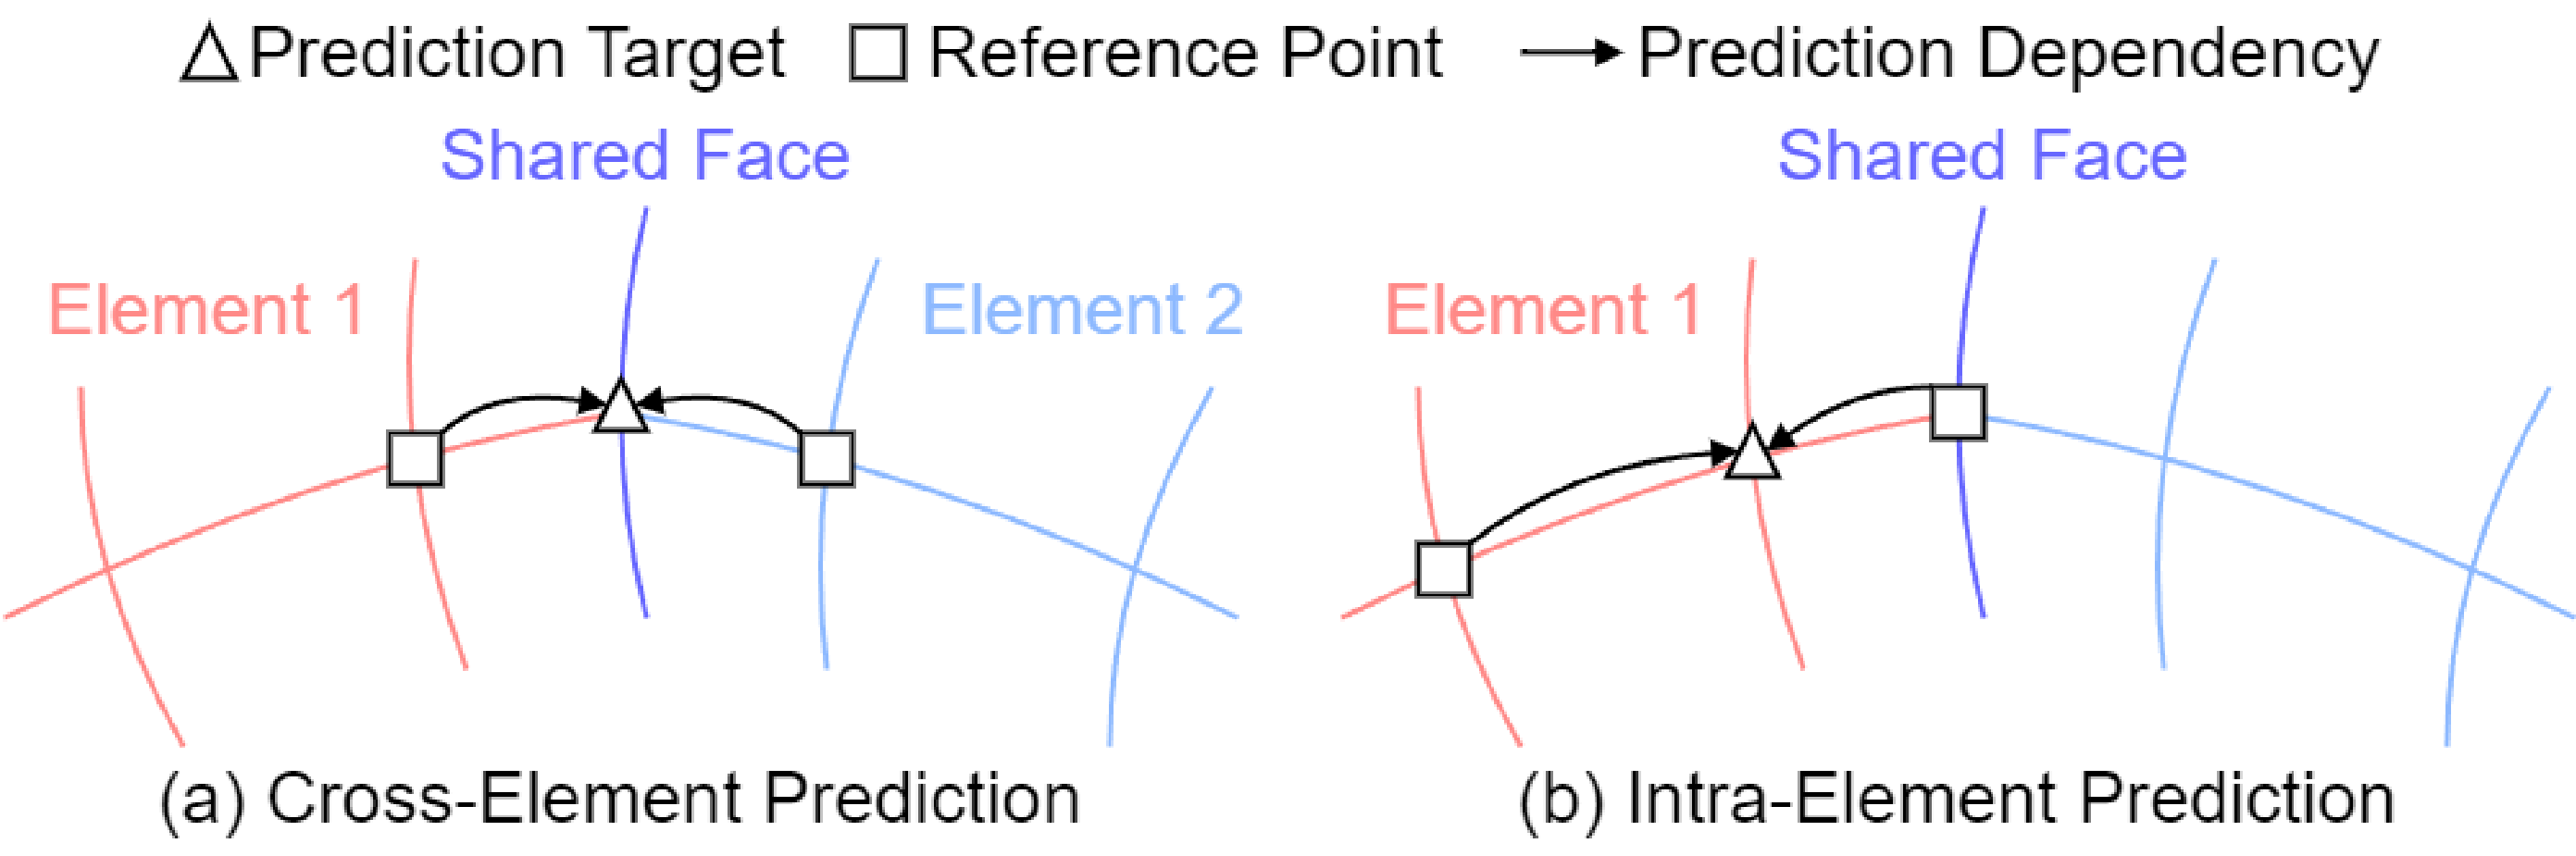
\includegraphics[width=1\linewidth]{figs/5/cross-element.pdf}
    \caption{Illustration of the Point Configurations Used in Cross-Element and Intra-Element Prediction}
    \label{fig:cross-element}
\end{figure}

We further explain the rationale for using intra-element prediction instead of cross-element prediction in FDWZ. In principle, cross-element prediction may benefit from the dense sampling near element boundaries. Since the physical distance between points across a shared face is small, their values may be more similar than those of neighboring points closer to the element interior, which can improve prediction accuracy. However, the reference points used in cross-element prediction are generally not collinear with the prediction target in physical space, which can reduce the effectiveness of linear interpolation. By contrast, the target and reference points used for intra-element prediction are collinear in the reference element and remain nearly collinear in physical space, with only minor distortion introduced by the element mapping. These competing effects make it unclear a priori which strategy provides more accurate predictions. We therefore perform an empirical comparison of cross-element and intra-element prediction.

We conduct experiments on the NekRS dataset~\cite{fischer2022nekrs} with an element size of $8\times8\times8$ (Dataset 4 in Table~\ref{tab:datasets}). We randomly sample a subset of elements, identify their neighboring elements, and align the neighboring elements to ensure consistent face orientations. For cross-element prediction, each point on the shared face is treated as a prediction target, and one neighboring interior grid point from each of the two adjacent elements is used as a reference for weighted linear interpolation. For comparison, the intra-element scheme predicts the same target using two reference points from the same element, both selected along the grid line extending from the shared face into the element interior. In both cases, prediction accuracy is quantified using mean squared error (MSE).

% \begin{table}[h]
%     \caption{MSE between cross-element and intra-element predictions across five faces of element 1940839.}
%     \label{tab:cross-element mse}
%     \centering
%     \begin{tabular}{c|cc}\toprule
%         \textbf{Adjacent Element} & \textbf{Cross-Element MSE} & \textbf{Intra-Element MSE} \\\midrule
        
%         1940803 & 2.049e-09 & 1.842e-08 \\
%         1940840 & 6.993e-04 & 1.146e-05\\
%         1940827 & 2.695e-07 & 3.909e-07\\
%         1940833 & 4.341e-08 & 2.526e-07\\
%         1940849 & 7.868e-06 & 1.031e-06\\\bottomrule
%     \end{tabular}
% \end{table}

\begin{table}[h]
    \caption{Comparison of Cross-Element and Intra-Element Prediction MSEs of a Representative Element}
    \label{tab:cross-element mse}
    \centering
    \begin{tabular}{c|cc}\toprule
        \textbf{Face Index} & \textbf{Cross-Element MSE} & \textbf{Intra-Element MSE} \\\midrule
        1 & 2.049e-09 & 1.842e-08 \\
        2 & 6.993e-04 & 1.146e-05\\
        3 & 2.695e-07 & 3.909e-07\\
        4 & 4.341e-08 & 2.526e-07\\
        5 & 7.868e-06 & 1.031e-06\\\bottomrule
    \end{tabular}
\end{table}

Table~\ref{tab:cross-element mse} presents the results for a representative element with five faces that have adjacent elements. Its remaining face has no identifiable adjacent element and is therefore excluded from the comparison. Additional tests show that either cross-element or intra-element prediction may achieve lower MSE on an individual face, while their average MSEs over a large number of faces are comparable. Thus, cross-element prediction provides no consistent accuracy advantage to justify the additional overhead of connectivity identification and orientation alignment. We therefore adopt intra-element prediction in FDWZ.
